%!TEX root = ../TAMUTemplate.tex
%%%%%%%%%%%%%%%%%%%%%%%%%%%%%%%%%%%%%%%%%%%%%%%%%%%
%
%  New template code for TAMU Theses and Dissertations starting Fall 2016.
%
%  Author: Sean Zachary Roberson
%    Version 3.16.09
%  Last updated 9/12/2016
%
%%%%%%%%%%%%%%%%%%%%%%%%%%%%%%%%%%%%%%%%%%%%%%%%%%%

%%%%%%%%%%%%%%%%%%%%%%%%%%%%%%%%%%%%%%%%%%%%%%%%%%%%%%%%%%%%%%%%%%%%%%%
%%%                           SECTION II
%%%%%%%%%%%%%%%%%%%%%%%%%%%%%%%%%%%%%%%%%%%%%%%%%%%%%%%%%%%%%%%%%%%%%%

\chapter{\uppercase {Theoretical Framework}}
\label{ch:theoretical_framework}

Since the mid-1970s, the Standard Model (SM) of particle physics has been the leading theory describing three of the four known fundamental forces (not including gravity) as well as classifying all of the known elementary particles.
Even during it's formative years, the SM's success at predicting new particles (i.e. the top quark in 1995) and describing the properties of known particles (i.e. $W^{\pm}$ to $Z^{0}$ mass ratio) was undeniable.
The model's roots can be traced back to 1930 when Herman Weyl was able to describe electromagnetism as a local symmetry represented by the Lie group $U\left(1\right)$~\cite{Weyl1929}.
In 1954 Yang and Mills created a theory which tried to extend the idea of gauge theory to non-abelian groups~\cite{PhysRev.96.191}.
This laid the ground work for Sheldon Glashow to combine the electromagnetic and weak interactions in 1961~\cite{GLASHOW1961579}.
This combined interaction is described by the $SU\left(2\right){\times}U\left(1\right)$ group.
In 1967 Steven Weinberg and Abdus Salam~\cite{PhysRevLett.19.1264,salam1968} continued this work by adding in the Higgs mechanism first proposed by Brout, Enlert Higgs, Guralnik, Hagen, and Kibble~\cite{PhysRevLett.13.321,PhysRevLett.13.508,Higgs:1966ev,PhysRevLett.13.585,Kibble:1967sv}.
The model entered its current form in 1973-1974 with the introduction of the strong force and quantum chromodynamics (QCD)~\cite{Neeman:1961jhl,GellMann:1962xb,GellMann:1964nj,Zweig:1981pd,Fritzsch:1972jv}.
The full theory is described by the symmetry group
\begin{equation}\label{eq:standard_model_symmetry_group}
SU\left(3\right)_{C}{\otimes}SU\left(2\right)_{L}{\otimes}U\left(1\right)_{Y}
\end{equation}
where $SU\left(2\right)_{L}{\otimes}U\left(1\right)_{Y}$ is the electroweak symmetry group describing both the electromagnetic and weak interactions and $SU\left(3\right)_{C}$ is the symmetry group describing the strong interaction~\cite{Burgess2007,Aitchison2012}.
\begin{comment}
$U\left(1\right)_{Y}$ for electromagnetic interactions, 
	one spin-1 field ($B^{\mu}$)
$SU\left(2\right)_{L}$ for weak interactions among fermions, 
	group has 3 spin-1 fields ($W_{a}^{\mu}$ where $a=1,2,3$)
$SU\left(3\right)_{C}$ describes colored QCD interactions
	group has 8 generators = eight spin-1 gluon fields ($G_{a}^{\mu}$ where $a=1,...,8$)
\end{comment}

The rest of this chapter will discuss the standard model, both its structure and some of its mathematical underpinnings, in more detail.
Section~\ref{sec:standard_model} will introduce the particle content of the SM.
The QFTs that govern the SM interactions will be discussed in sections~\ref{sec:QED} to~\ref{sec:higgs_mechanism}.
Given the more detailed explanation, a short summary of the SM will be given in~\ref{sec:standard_model_summary}.
In section~\ref{sec:BSM} we will briefly reference how Higgs physics can relate to physics beyond the SM.

\section{The Standard Model}
\label{sec:standard_model}

The standard model is a locally guage-invariant quantum field theory (QFT) in four-dimensional Minkowski space~\cite{Burgess2007,Barnes2010}.
The structure and particle content of the SM can be found in fig~\ref{fig:standard_model}.
The SM is composed of 12 fermions, the particles that make up matter, and 4 gauge bosons, the force-carrying particles which mediate the electromagnetc, weak, and strong interactions.
On its own, the basic symmetries of the standard model require that the guage bosons (W$^\pm$,Z,$\gamma$,gluons) be masseless.
However, we know that this is not true as experiments have shown that the $W$ and $Z$ bosons have quite a large mass.
The afformentioned Higgs mechanism takes care of this by spontaneously breaking the electroweak symmetry, giving mass to the quarks, the leptons, and the $W$ and $Z$ bosons~\cite{PhysRevLett.19.1264,salam1968,Dawson:1998yi}.

\begin{figure}[!hbt]
	%\scalebox{.45}{\input{StandardModel}}
	\centering
	\resizebox{0.95\textwidth}{!}{\input{StandardModel_CERNWebfest2012}}
	\caption{The Standard Model of particle physics. The model includes three generations of matter particles (leptons and quarks) as well as the gauge and Higgs bosons. Included in this drawing are the particle names, symbols, masses, spin, electric charge, and color charge, if applicable.}
	\label{fig:standard_model}
\end{figure}

Fermions are particles which obey Fermi-Dirac statistics and the Pauli exclusion principle, meaning that no two fermions may occupy the same quantum state within a given quantum system.
These particles have half-integer spin, often denoted as spin-1/2 particles, which means that their intrinsic angular momentum is $\hbar/2$.
For every fermion $f$ in the SM there exists an anti-fermion $\bar{f}$, which has an identical mass, but opposite quantum numbers.
The fermions in the SM are separated into six leptons and six quarks with these further separated into 3 generations of pairs of particles.
Each subsequent generation is ostensibly a heavier version of the previous generation, with the same quantum numbers.\footnote{The neutrinos may have a different mass ordering.}

Each generation of lepton can be broken down into a charged and neutral lepton.
For instance, the first generation is composed of the electron (\Pe), with charge $-\Pe$, and the electron neutrino ($\Pgn_{e}$).
The second and third generations contain the muon (\Pmu) and tau (\Ptau) along with their associated neutrinos.
Although the SM specifies that the neutrinos are massless, experiments have shown that this is not true.
While their exact masses are still unknown, upper bounds have been places on these and can be seen in fig~\ref{fig:standard_model}.
Each generation of lepton has an associated quantum number, called the lepton number, defined as $L_{\ell}=n_{\ell}-n_{\bar{\ell}}$.
First generation leptons have quantum numbers $L_{e}=+1$ and $L_{\mu}=L_{\tau}=0$ while the second and third generations have value $+1$ for their associated lepton number and zero otherwise.
The antileptons have oppositely signed lepton numbers.
The lepton numbers are a conserved quantity in the SM, which means that only lepton-antilepton pairs can be created or destroyed.\
That being said, neutrino oscillations, the phenomina of neutrinos changing flavor from one generation to the next, has been observed~\cite{Maltoni:2004ei}.
While this violates the conservation of lepton numbers within a generation, the total lepton number $L{\equiv}L_{e}+L_{\mu}+L_{\tau}$ may still be conserved.
All leptons interact through the wek interaction, but only the charged leptons interact using the electromagnetic interaction.
Because leptons lack the color charge they do not interact using the strong force.

Like the leptons, the three generation of quarks can be broken into one up-type quark and one down-type quark, categories which gain their name through the content of the first generation containing the up (\cPqu) and down (\cPqd) quarks.
The second generation is made up of the charm (\cPqc) and strange (\cPqs) quarks while the third is made up of the top (\cPqt) and bottom (\cPqb) quarks.
The up-type quarks have fractional electric charge of $Q=+2e/3$ and the bottom-type quarks have electric charge $Q=-e/3$.
As in the case of the leptons, the quarks have an associated baryon quantum number, $B$.
This quantity is conserved in all SM interactions and no exception has every been seen.
This means that only quark-antiquark pairs may be created or destroyed and also results in the stability of the lightest baryon, the proton.
Baryon number is defined as $B=\frac{1}{3}\left(n_{q}-n_{\bar{q}}\right)$, where, for example, the baryon number for a quark is $+1/3$ and $-1/3$ for an antiquark.
Quarks may interact through the electromagnetic and weak interactions, but unlike the lepton, quarks can also interact via the strong force.
This is because quarks also have color charge, which can have three values referred to as red, green, or blue. 
Antiquarks may contain charges of anti-red, anti-green, or anti-blue.
In the SM colorless particles are forbidden from existing on their own, which means that individual quarks, often refered to as bare quarks, have never been seen in nature.
Instead, quarks are always found as constituents of bound states called hadrons.
This group of composite particles may be further divided into mesons, bound states of a quark-antiquark pair, and baryons, bound states of three quarks and antiquarks.
The hadrons contain quark and antiquark combinations such that the bound state is a color singlet, often referred to as being colorless.
Mesons contain color-anticolor pairs while baryons consist of red, green, and blue charged quarks.
The masses of the quarks are hard to measure due to their confinement in hadrons, however, global averages have been made.

\section{Quantum Electrodynamics}
\label{sec:QED}

Quantum electrodynamic (QED) is a quantum field theory which describes the dynamics of the electromagnetic interaction.
In a QFT, particles are represented by fields, which are in turn reresented mathematicaly by Lagrangian densities $\mathcal{L}$.
QED was formulated to described the interactions of spin 1/2 particles, namely leptons and quarks.
Like a classical field theory, the dynamics of a quantum system are described by a Lagrangian.
QED is described by the Dirac Lagrangian density
\begin{equation}\label{eq:dirac_lagrangian_density}
\mathcal{L}=i\bar{\psi}\gamma^{\mu}\partial_{\mu}\psi-m\bar{\psi}\psi
\end{equation}
where $\psi$ a four-component column vector representing the wave function of a spin 1/2 particle\footnote{$\psi$ is a field known as a Dirac spinor.}, $\gamma^{\mu}$ are the four Dirac gamma matrices, $\bar{\psi}\equiv\psi^{\dagger}\gamma^{0}$, and $m$ is the mass of the particle.



QED must be invariant under local and global gauge transformations
global $U\left(1\right)$ transformation:
	\begin{equation}\label{eq:global_u1_transformation}
		\psi\rightarrow\psi'=e^{-i\alpha}\psi
	\end{equation}
	$\alpha$ is a constant
	Replace $\psi$ in~\ref{eq:dirac_lagrangian_density} by~\ref{eq:global_u1_transformation} and $\mathcal{L}\rightarrow\mathcal{L}'=\mathcal{L}$
	So it is invariant under this type of transformation
local transformation $\alpha\rightarrow\alpha\left(x\right)$ where $\alpha$ is allowed to vary as a function of spacetime:
	then~\ref{eq:global_u1_transformation} becomes a local $U\left(1\right)$ transformation
	then equation~\ref{eq:dirac_lagrangian_density} becomes
	\begin{equation}\label{eq:local_transformation}
		\mathcal{L}\rightarrow\mathcal{L}'=\mathcal{L}+\bar{\psi}\gamma^{\mu}\left(\partial_{\mu}\alpha\left(x\right)\right)\psi
	\end{equation}
	thus not invariant under this transformation.
	to return invariance replace partial derivative in Lagrangian density by covariant derivative
	\begin{equation}\label{eq:covariant_derivative}
		D_{\mu}=\partial_{\mu}+iqA_{\mu}
	\end{equation}
	$q=-e$ is the electron charge (in case of an electron)
	$A_{\mu}$ is a new gauge field representing the photon, the mediator of electromagnetic interactions, and transforms as
	\begin{equation}\label{eq:photon_transformation}
		A_{\mu}{\rightarrow}A_{\mu}'=A_{\mu}+\partial_{\mu}\chi\left(x\right)
	\end{equation}
	$\chi\left(x\right)$ is an arbitarary function of spacetime.
	when gauge transformation~\ref{eq:global_u1_transformation} is made to lepton field and~\ref{eq:photon_transformation} is made to photon field and $\chi\left(x\right)=\alpha\left(x\right)/q$ the covariant derivative transforms in the same way as $\psi\left(x\right)$, namely $D_{\mu}\psi\rightarrow\left(D_{\mu}\psi\right)'=e^{-i\alpha}D_{\mu}\psi$

	After the changes listed above, equation~\ref{eq:dirac_lagrangian_density} will take the locally gauge invariant form
	\begin{equation}\label{eq:dirac_lagrangian_density_local_invariant}
		\mathcal{L}=\bar{\psi}\left(i\gamma^{\mu}D_{\mu}-m\right)\psi-\frac{1}{4}F^{\mu\nu}F_{\mu\nu}
	\end{equation}
	where
	\begin{equation}\label{eq:electromagnetic_field_strength_tensor}
		F^{\mu\nu}=\left(\partial^{\mu}A^{\nu}-\partial^{\nu}A^{\mu}\right)
	\end{equation}
	is the electromagnetic field strength tensor
	no $m^{2}A_{\mu}A^{\mu}$ term, which would be the mass of the gauge field, but the photon is massless
	in the case of an electron, for example, it does contain an $e^{+}e^{-}\gamma$ interaction and a term quadritic in the fireld strength tensor, which is the photon kinetic energy 
	eqn~\ref{eq:dirac_lagrangian_density_local_invariant} describes lepton interactions
	Complete QED Lagrangian can be created by generalizing to all leptons by $\psi\rightarrow\psi_{i}$ and summing over all leptons $i=e,\mu,\tau,u,d,c,s,t,b$ as in equation~\ref
	\begin{equation}\label{eq:qed_lagrangian}
		\mathcal{L}=\sum_{i}\left[\bar{\psi}_{i}\left(i\gamma^{\mu}D_{\mu}-m_{i}\right)\psi_{i}\right]-\frac{1}{4}F_{\mu\nu}F^{\mu\nu}
	\end{equation}

\begin{comment}
Bosons:
electromagnetic interaction = $\gamma$, corresponds to the $U_{EM}\left(1\right)$ group, massless and no electric charge Q. Infinite range because photon is massless. Quantum electrodynamics (QED) is a gauge-invariant QFT that describes electromagnetism and will be discussed more in section~\ref{sec:QED}
weak interaction
	correspond to the broken part of $SU_{L}\left(2\right){\times}U_{Y}\left(1\right)$ group
	weak force acts on particles carrying weak isospin $T$
	only left-handed fermions have weak isospin
	Third component of isospin quantum number, $T_{3}$, is always conserved
	massive bosons, so weak force has a range of about $10^{-18}\unit{m}$
	charged weak interaction = W$^\pm$
		only left-handed fermions and right-handed antifermions sensitive to charged weak interactions (chirality is important)
	neutral weak interaction = Z
		acts on all fermions of all chiralities, but coupling strength does depend on chirality

can unify the electromagnetic and weak forces into the symmetry group
\label{eq:electroweak_interaction_group}
	SU_{L}\left(2\right){\times}U_{Y}\left(1\right)
\end{equation}
a new conserved quantum number, weak hypercharge, is formed from the quantum number of electromagnetism and weak forces: $Y=2\left(Q-T_{3}\right)$

Higgs responsible for electroweak symmetry breaking (EWSB), discussed more in section~\ref{sec:higgs_mechanism}
	For electroweak interaction to be gauge invariant the gauge bosons corresponding to this force must be massless, which they aren't.
	Higgs mechanism solves this.
	Short version is that Higgs field causes a spontaneuous EWSB due to its non-zero vacuum expectation value (VEV)
	\begin{equation}
	\label{eq:spontaneous_symmetry_breaking}
	SU_{L}\left(2\right){\times}U_{Y}\left(1\right){\rightarrow}U_{EM}\left(1\right)
	\end{equation}
	allows fermion field to aquire mass, which it was forbidden to do from eqn.~\ref{eq:standard_model_groups}
	Higgs field contains a doublet of scalar bosons, two charged particles and two neutral particles.
		Two charged and one neutral combine with W$^{\pm}$ and Z to produce their masses
		Other neutral particle is the Higgs boson H
	Higgs boson 

strong interaction = gluon
	from $SU\left(3\right)_{C}$ group, massless and have color, but no electric charge Q
	range is about $10^{-15}\unit{m}$
	quarks are confined particles, meaning that the attractive force between them does not decrease as they more farther apart.
	instead the force decreases as the particles move closer and increases as they move farther apart
	this behavior is called asymptotic freedom
	as the energy in the gluon field between quarks increases it can become large enough to form a quark-antiquark pair, preventing the original quarks from being in a bare state
	formation of a bound state called hadronization
	strong force also responsible for acting on nucleons, i.e. protons and neutrons, to form atomic nuclei.


SM Lagrangian density
\begin{equation}
\label{eq:SM_Lagrangian_density}
\ell_{SM}=\ell_{kinetic}+\ell_{Yukawa}+\ell_{Higgs}
\end{equation}
$\ell_{kinetic}$ = kintetic terms plus gauge interactions
\ell_{Yukawa} = contains terms coupling fermion fields to Higgs fields
\ell_{Higgs} = related to Higgs potential $V\left(\phi\right)$, through $\ell_{Higgs}=-V\left(\phi\right)$ where
\begin{equation}
\label{eq:Higgs_potential}
V\left(\phi\right)=-\mu^{2}|\phi^{\dagger}\phi|+\lambda\left(|\phi^{\dagger}\phi|\right)^{2}
\end{equation}
with $\mu^{2}>0$ and $\lambda>0$
Higgs potential minimized at non-zero value of Higgs field
	nonzero ground state or vacuum expectation value (vev)
	may be chosen so that real, enutral componenet is non-zero
	\begin{equation}
	\left<\phi\right>=\frac{1}{\sqrt{2}}\left(\begin{array}{c}0 \\\nu\end{array}\right)
	\end{equation}
	where $\nu^{2}=\frac{\mu^{2}}{\lambda}$
	vev is source of electroweak symmetry breaking.

If forces weak enough, can QFT calculations use perturbative method to calculate leading order (LO) term.
next-to-leading order (NLO) corretions added in, then next-to-next-to leading order (NNLO) and so on
\end{comment}





\section{Electroweak Interaction}
\label{sec:electroweak_interaction}
\section{Strong Interaction}
\label{sec:strong_interaction}
\section{Higgs Mechanism}
\label{sec:higgs_mechanism}

\begin{comment}
\begin{figure}[!hbt]
    \centering
    \begin{subfigure}[t]{0.48\textwidth}
        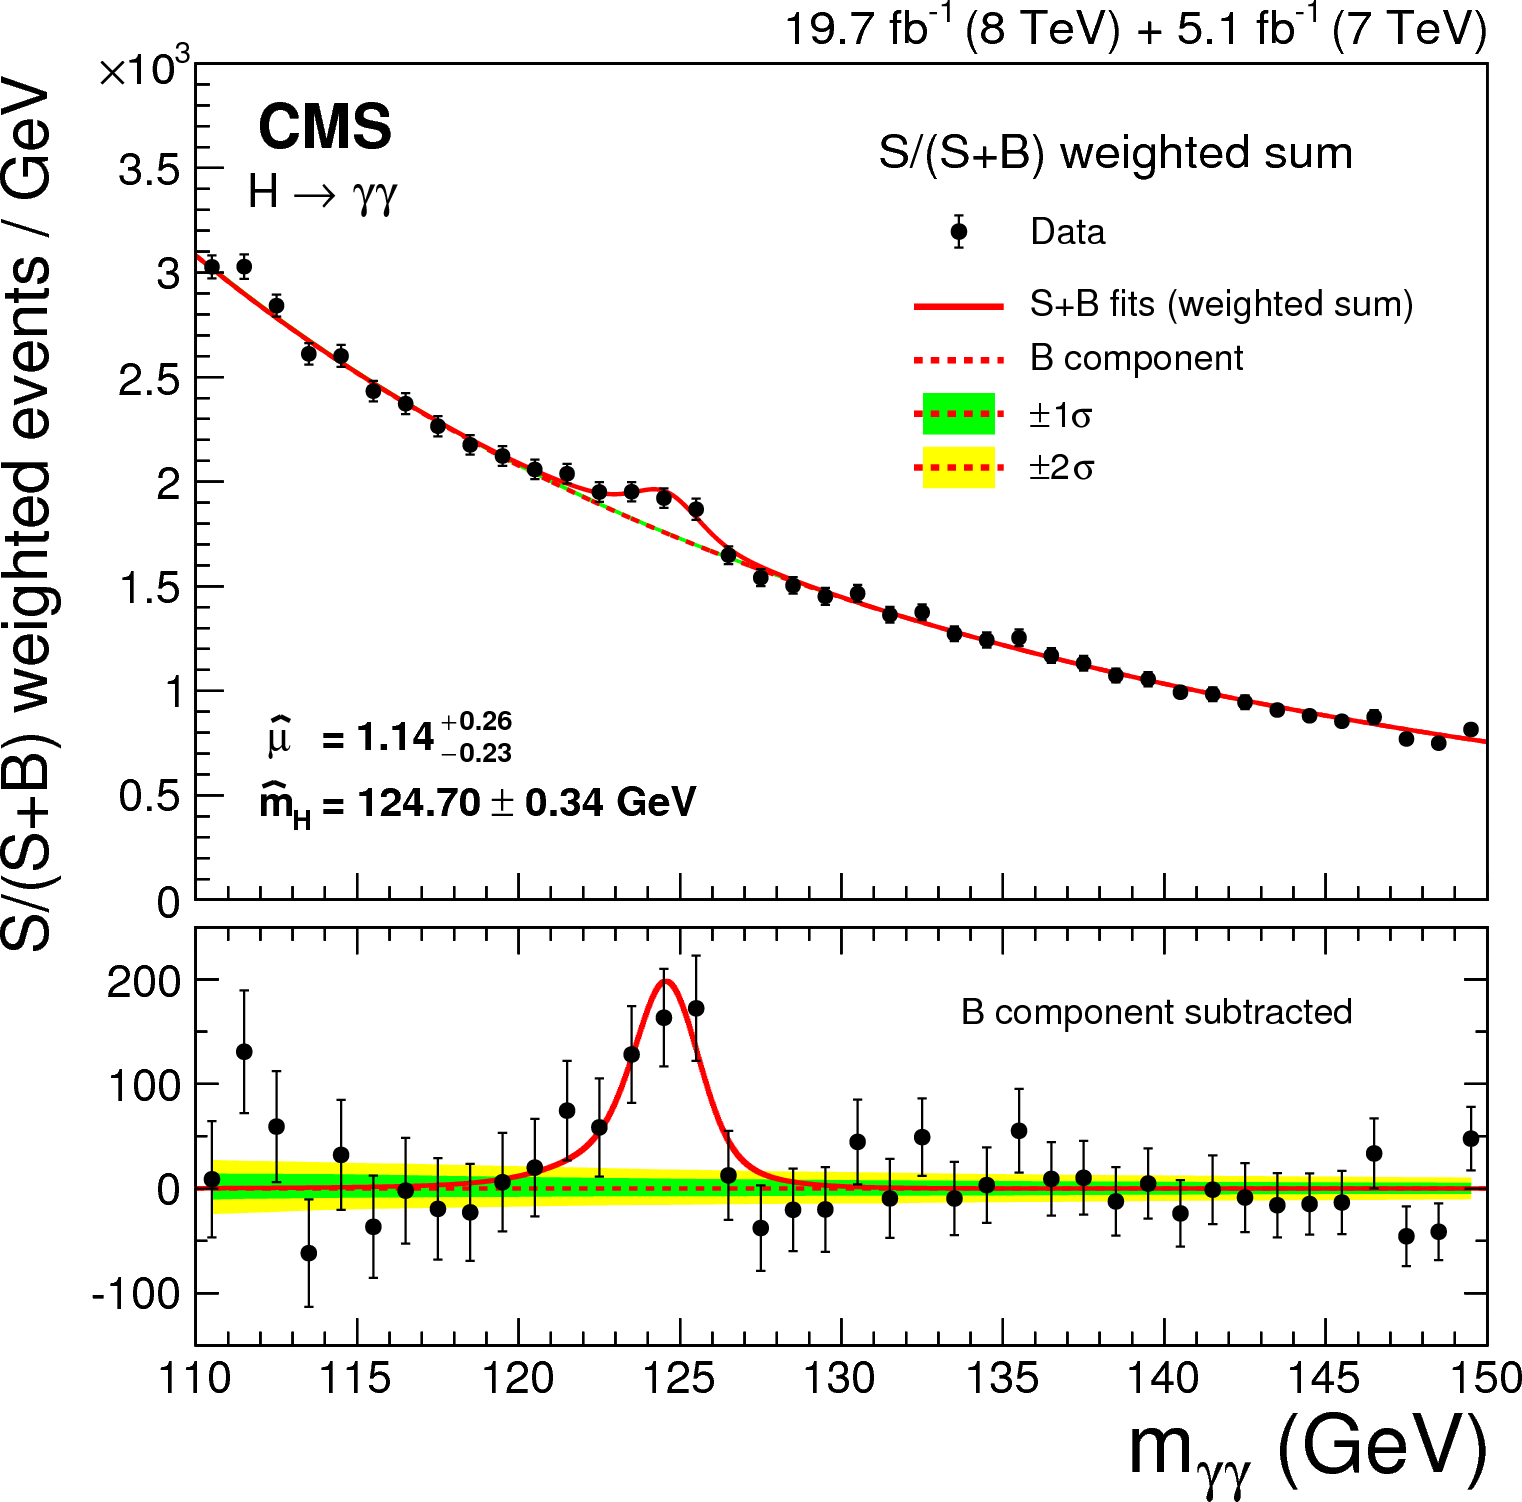
\includegraphics[width=\textwidth]{\figpath/Chapter2/HgammagammaPeak.png}
        \caption{}
        \label{fig:HgammagammaPeak}
    \end{subfigure}
    \begin{subfigure}[t]{0.48\textwidth}
        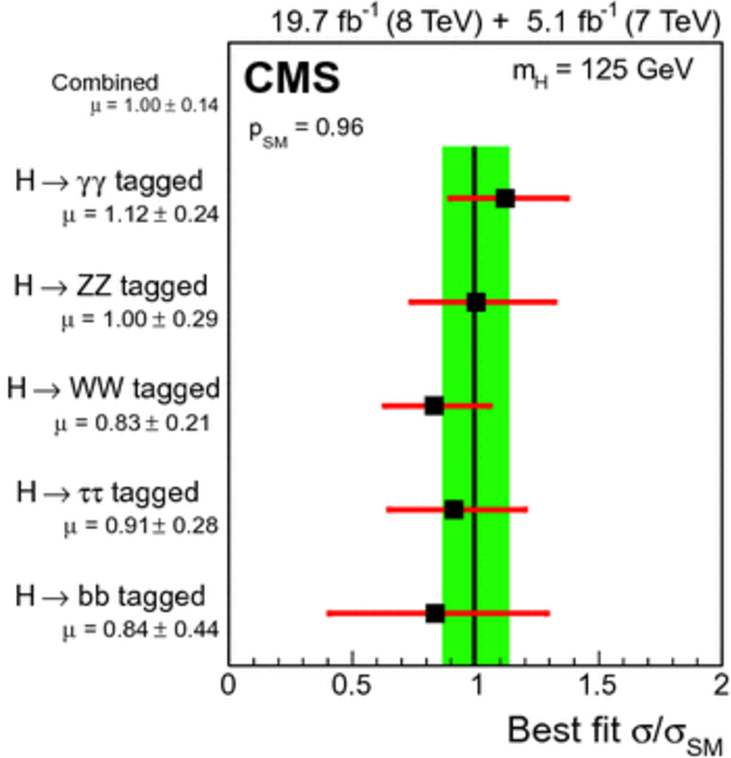
\includegraphics[width=\textwidth]{\figpath/Chapter2/10052_2015_3351_Fig4_HTML.pdf}
        \caption{}
        \label{fig:HiggsSignalStrength}
    \end{subfigure}
    \caption{(Left) The $H\rightarrow\gamma\gamma$ signal peak as seen in 2012~\cite{Hgammagamma}. (Right) Best-fit $\sigma/\sigma_{SM}$ grouped by predominant decay mode. The vertical band is the overall combined analysis value and the horizontal bars show the $\pm$1 uncertainties (statistical and systematic)~\cite{Khachatryan2015}.}
    \label{fig:HiggsIn2012}
\end{figure}
\end{comment}

%, as seen in figure~\ref{fig:Higgs_WW_lnujj_feynman}

%While at 125\gev the gluon-gluon fusion (ggF) production cross section\footnote{This analysis is independent of production mode, but selects for a specific decay channel.} and $l\nu{qq}$ branching ratio are high, as seen in figure~\ref{fig:Higgs_XS_and_BR}, there are significant experimental challenges to overcome.

\begin{comment}
\begin{figure}[bt]
	\centering
	\begin{subfigure}[t]{0.415\textwidth}
		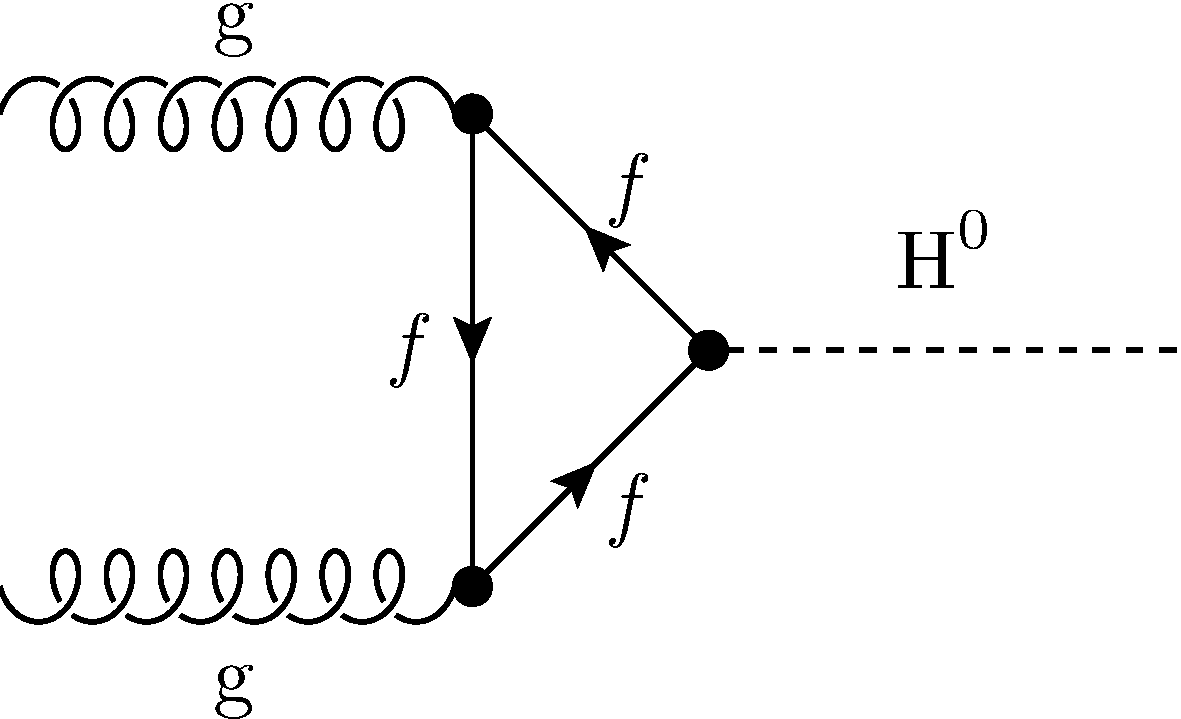
\includegraphics[width=\textwidth]{\figpath/FeynmanDiagrams/ggH.eps}
		\label{fig:ggH}
	\end{subfigure}%
	\begin{subfigure}[t]{0.415\textwidth}
		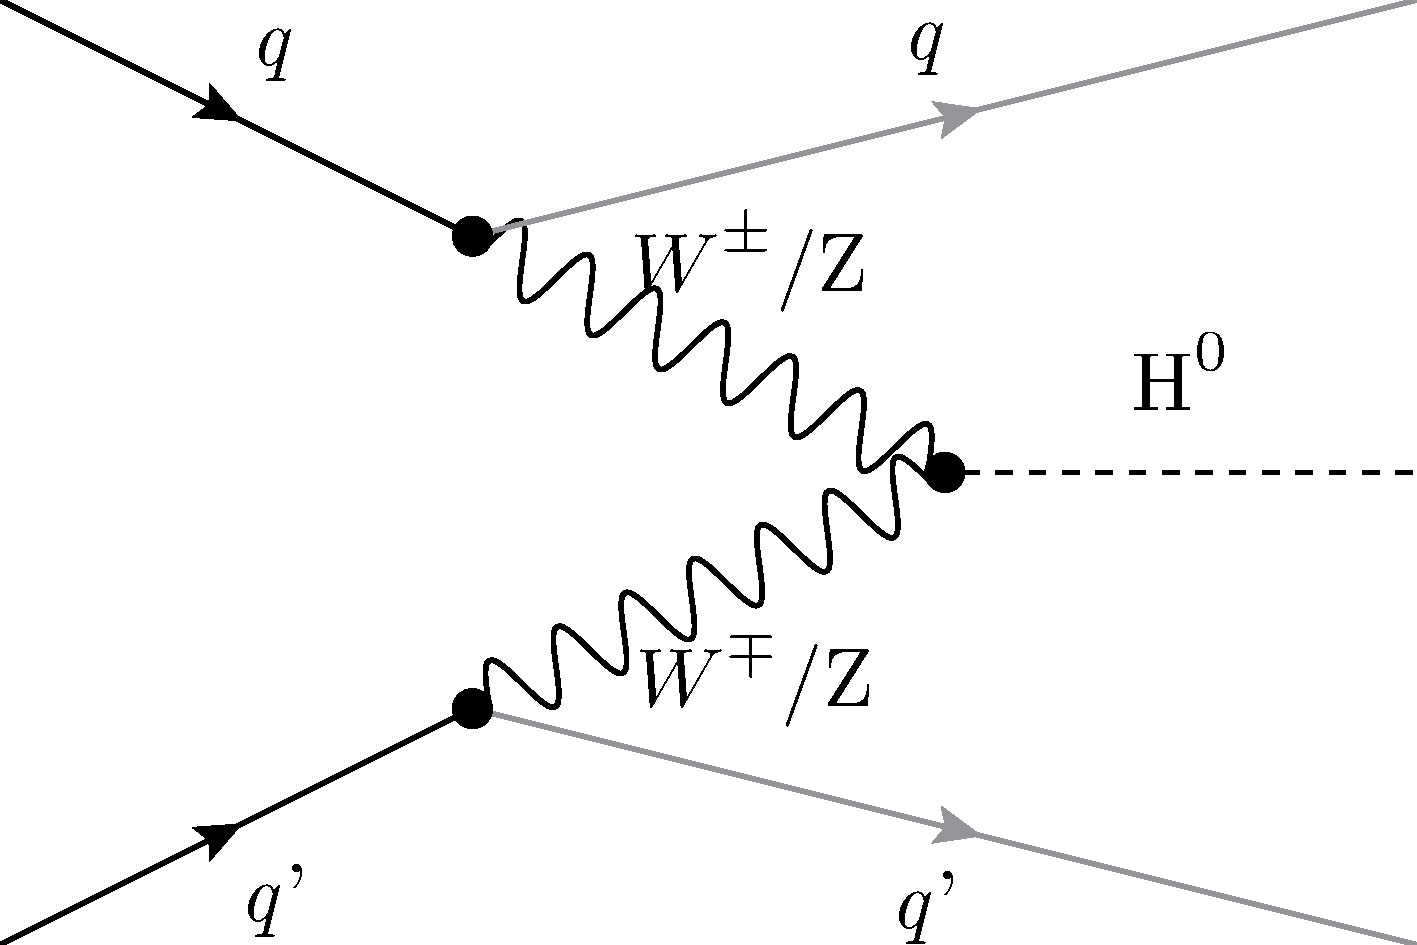
\includegraphics[width=\textwidth]{\figpath/FeynmanDiagrams/qqH.eps}
		\label{fig:qqH}
	\end{subfigure}

	\begin{subfigure}[t]{0.415\textwidth}
		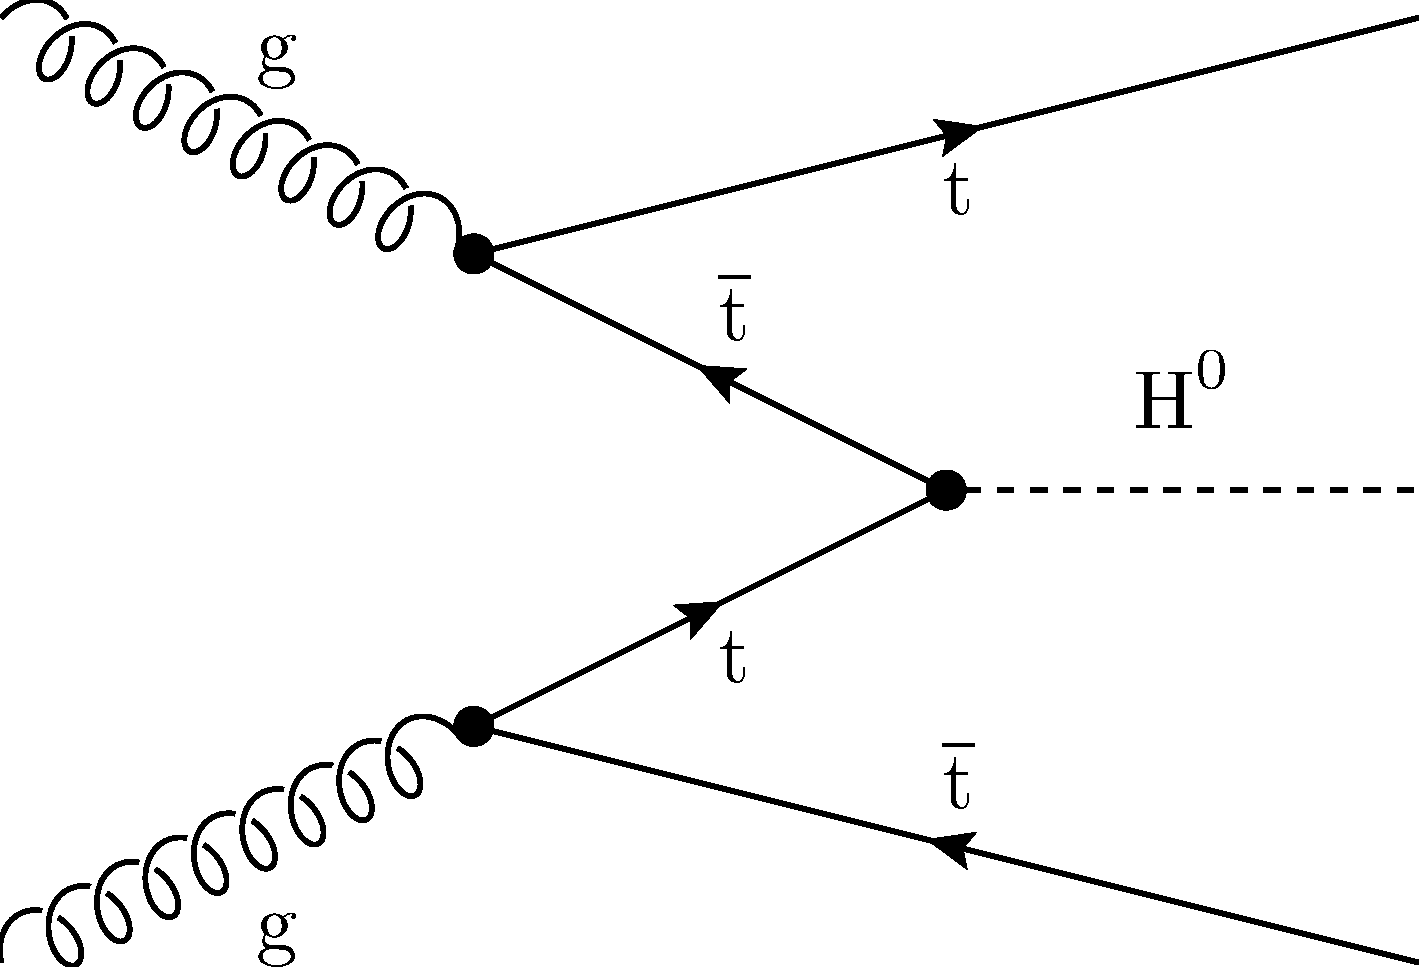
\includegraphics[width=\textwidth]{\figpath/FeynmanDiagrams/ttH.eps}
		\label{fig:ttH}
	\end{subfigure}%
	\begin{subfigure}[t]{0.415\textwidth}
		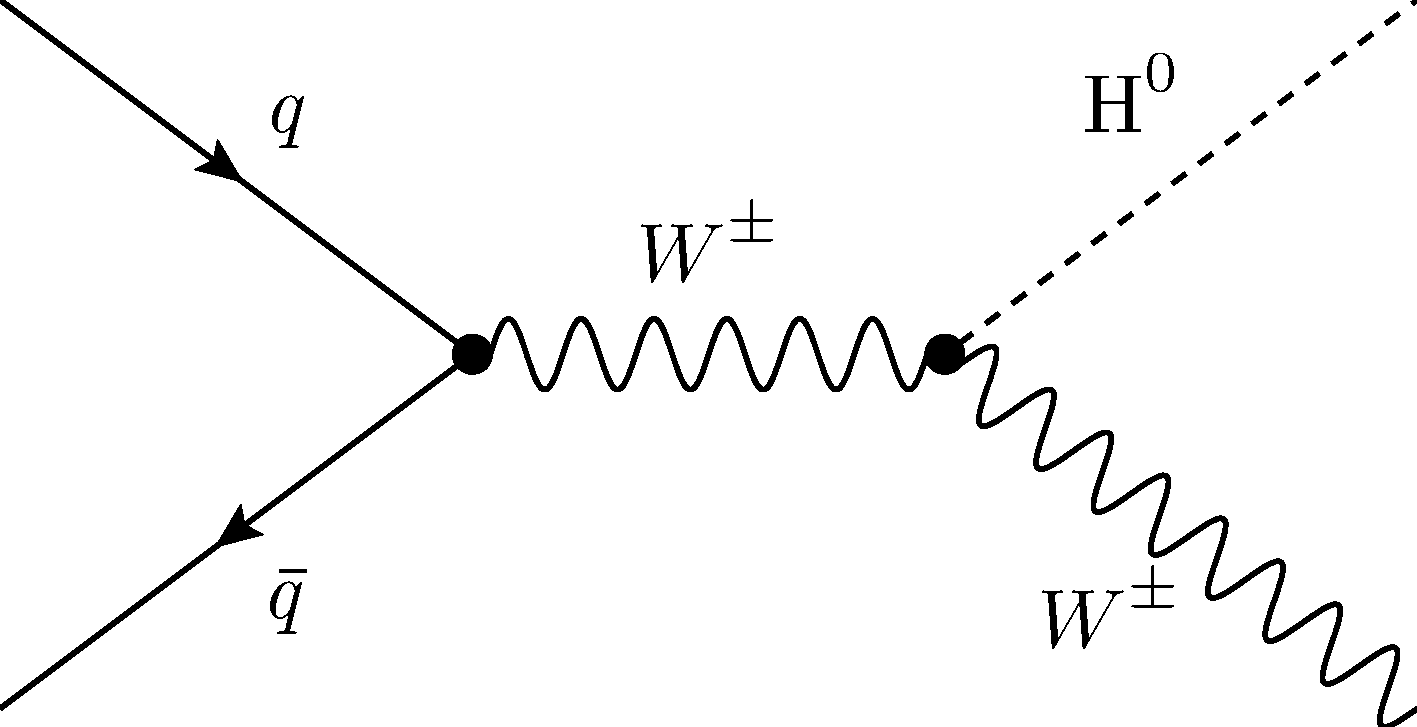
\includegraphics[width=\textwidth]{\figpath/FeynmanDiagrams/WH.eps}
		\label{fig:WH}
	\end{subfigure}
	\caption{Feynman diagrams for the four Higgs production mechanisms with associated $l{\nu}qq$ decays: gluon-gluon fusion (upper left), vector-boson fusion (upper right), \ttbar fusion (lower left), and associated production (lower right).}
	\label{fig:Higgs_WW_lnujj_feynman}
\end{figure}

\begin{figure}[!hbt]
	\centering
	\begin{subfigure}[t]{0.54\textwidth}
		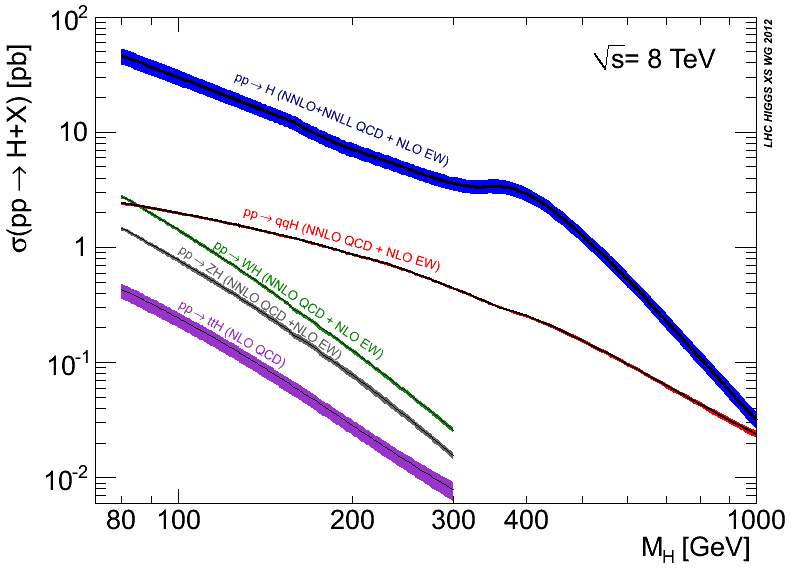
\includegraphics[width=\textwidth]{\figpath/Chapter2/Higgs_XS_8TeV.png}
		\label{fig:Higgs_XS_8TeV}
	\end{subfigure}
	\begin{subfigure}[t]{0.41\textwidth}
		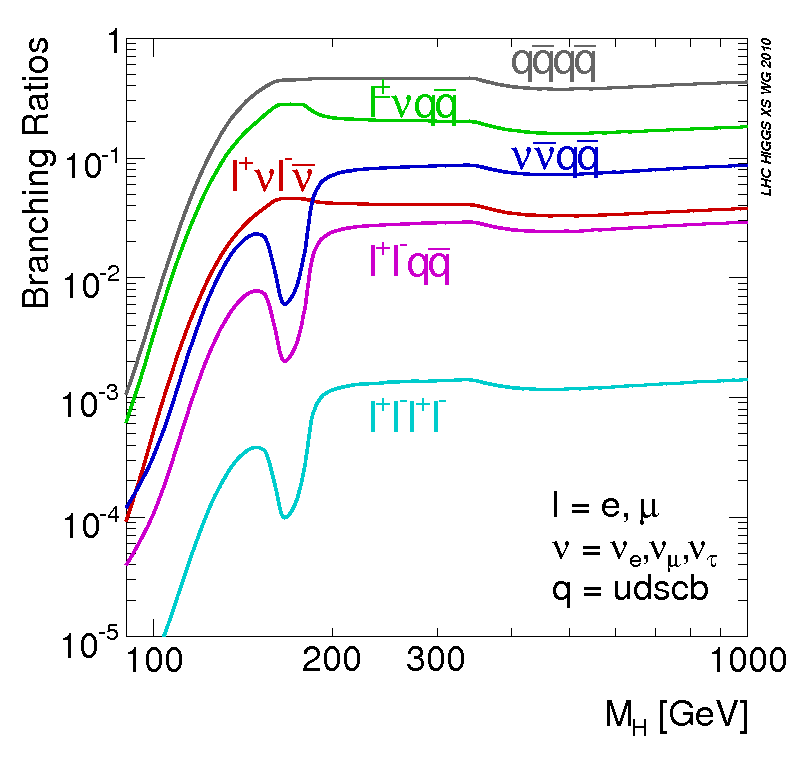
\includegraphics[width=\textwidth]{\figpath/Chapter2/Higgs_BR_4fermion.png}
		\label{fig:Higgs_BR_4fermion}
	\end{subfigure}
	\caption{The Standard Model Higgs production cross sections at 8\tev (left) and WW branching ratios to four fermion final states (right).}
	\label{fig:Higgs_XS_and_BR}
\end{figure}
\end{comment}

\section{Global Picture}
\label{sec:standard_model_summary}

Leptons:
leptons have electric charge and weak isospin
neutrinos have only weak isospin

Quarks:
quarks have color charge, weak isospin and electric charge



Fermions can also be grouped based on their chirality.
The left-handed up- and down-type quarks form a weak doublet $q_{L}$ and the left-handed charged leptons and neutrinos form a separate weak doublet $\ell_{L}$.
The right-handed particles form weak singlets, but right-handed neutrinos and left-handed antineutrinos don't exist in the SM.
Table~\ref{tab:fermion_quantum_numbers} shows these groups along with their associated quantum numbers.

\begin{table}[htbp]
	\caption{The quantum numbers of the SM fermions grouped by chirality and particle-type, independent of generation. The various particle-types in the SM are up-type quarks, down-type quarks, charged leptons, and neutrinos.}
	\centering
    \begin{tabular}{|l|l|r|r|r|r|r|}
\hline
      & \multicolumn{1}{c|}{Particle-Type} & \multicolumn{1}{c|}{$Q$} & \multicolumn{1}{c|}{$T_3$} & \multicolumn{1}{c|}{$Y$} & \multicolumn{1}{c|}{$B$} & \multicolumn{1}{c|}{$L$} \\
\hline
\multirow{3}{*}{Quarks}  
\rule{0pt}{24pt}         & $\cPq_L = \doublet[r]{\cPqu}{\cPqd}_L$ & $\doublet[r]{2/3}{-1/3}$ & $\doublet[r]{1/2}{-1/2}$ & $1/3$  & $1/3$ & 0 \\
                         & $\cPqu_R$                              & $2/3\hphantom{\bigg)}$   & $0\hphantom{\bigg)}$     & $4/3$  & $1/3$ & 0 \\
                         & $\cPqd_R$                              & $-1/3\hphantom{\bigg)}$  & $0\hphantom{\bigg)}$     & $-2/3$ & $1/3$ & 0 \\
\hline
\multirow{2}{*}{Leptons} 
\rule{0pt}{24pt}         & $\ell_L = \doublet[r]{\nu}{\Pe}_L$     & $\doublet[r]{0}{-1}$     & $\doublet[r]{1/2}{-1/2}$ & $-1$   & 0     & 1 \\
                         & $\Pe_R$                                & $-1\hphantom{\bigg)}$    & $0\hphantom{\bigg)}$     & $-2$   & 0     & 1 \\
\hline
    \end{tabular}
	\label{tab:fermion_quantum_numbers}
\end{table}


\begin{figure}[hbt]
	\begin{center}
		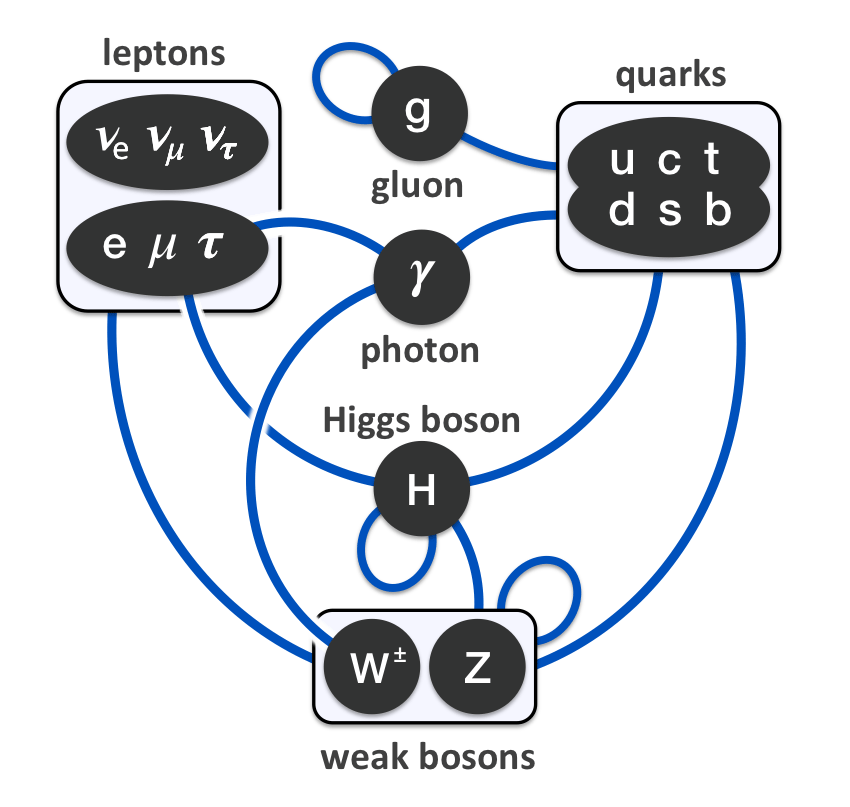
\includegraphics[width=0.95\textwidth]{figures/Chapter2/Elementary_particle_interactions_in_the_Standard_Model.png}
		\caption{A diagram illustrating the leading order interactions between particles in the standard model, including self-interactions~\cite{Drexler}.}
		\label{fig:sm-interactions}
	\end{center}
\end{figure}


\section{Beyond the Standard Model}
\label{sec:BSM}